\section{Visualization}

As a helpful utility, HOOVER offers basic support for visualizing HOOVER
simulations. Currently this support is limited to 2D simulations where there are
only two positional attributes for each actor. The HOOVER-viz tool will plot the
positions of each actor on a 2D plane for each timestep. It supports color
coding each actor by either the owning PE or by some attribute on the actor.

Visualizing a HOOVER simulation is a two-step process with online and offline
components. Online, HOOVER PEs generate traces of actor updates and write them
to disk as CSV files. This tracing is enabled whenever the environment variable
\texttt{HVR\_TRACE\_DUMP} is defined. Offline, the HOOVER-viz tool (which simply
consists of an HTML and Javascript file) reads the CSV files into your browser
and then plays back the activity on an HTML Canvas.

Figure~\ref{fig:hoover-viz} shows the HOOVER-viz tool. In the upper left corner
are controls for selecting a CSV to replay, toggling how to color code actors,
and resetting the simulation. In the upper right corner is a counter for the
current timestep. The remainder of the canvas is devoted to plotting actors.

\begin{figure}
\centering
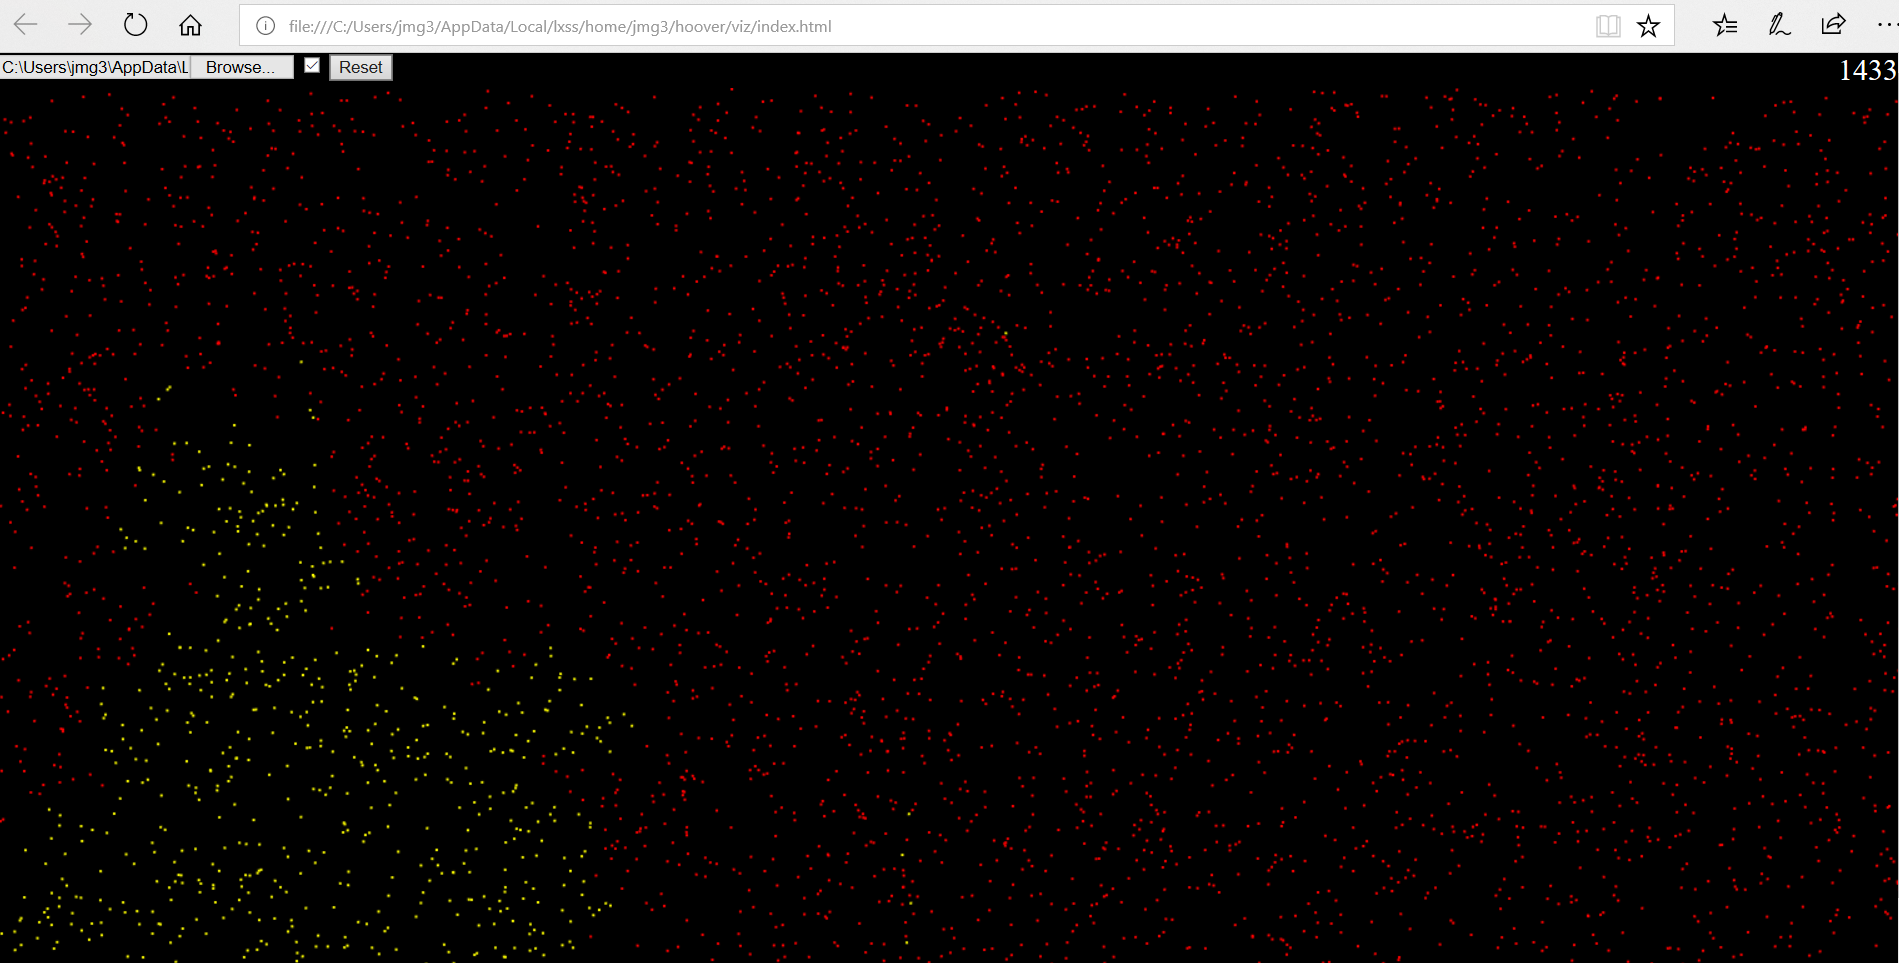
\includegraphics[width=\columnwidth]{hoover-viz.png}
\caption{Screenshot of the HOOVER-viz tool.}
\label{fig:hoover-viz}
\end{figure}

